%%%%%%%%%%%%%%%%%%%%%%%%%%%%%%%%%%%%%%%%%%%%%%%%%%%%%%%%%%%%%%%%%%%%%%%%%%%%%%%% 
%
%   Basic configuration
%
%%%%%%%%%%%%%%%%%%%%%%%%%%%%%%%%%%%%%%%%%%%%%%%%%%%%%%%%%%%%%%%%%%%%%%%%%%%%%%%%

% Use 'KOMA-Script Book' as the document class
\documentclass[toc=bibliography,toc=indentunnumbered,listof=totoc]{scrbook}



%%%%%%%%%%%%%%%%%%%%%%%%%%%%%%%%%%%%%%%%%%%%%%%%%%%%%%%%%%%%%%%%%%%%%%%%%%%%%%%%
%
%   Preload essentials
%
%%%%%%%%%%%%%%%%%%%%%%%%%%%%%%%%%%%%%%%%%%%%%%%%%%%%%%%%%%%%%%%%%%%%%%%%%%%%%%%%

% Load some required packages
\usepackage{etoolbox}                   % Modding standard environments
\usepackage[fleqn,intlimits]{amsmath}   % Common mathematical environments
\usepackage[svgnames]{xcolor}           % Enables coloring of text and pages
\usepackage{hyperref}                   % Enables hyperlink generation



%%%%%%%%%%%%%%%%%%%%%%%%%%%%%%%%%%%%%%%%%%%%%%%%%%%%%%%%%%%%%%%%%%%%%%%%%%%%%%%%
%
%   Page design
%
%%%%%%%%%%%%%%%%%%%%%%%%%%%%%%%%%%%%%%%%%%%%%%%%%%%%%%%%%%%%%%%%%%%%%%%%%%%%%%%%

% Font size
\KOMAoptions{fontsize=11pt}

% Line spacing
\linespread{1.04} 

% Paper format
\KOMAoptions{paper=B5}

% Duplex layout
\KOMAoptions{twoside}

% Page layout [1/sqrt(3)]
\usepackage[text={108.25mm,187.50mm},hmarginratio=1:1,vmarginratio=1:2]{geometry}

% Page layout [1/sqrt(2)]
%\KOMAoptions{BCOR=15mm}
%\KOMAoptions{DIV=11}

% Page layout [Classic circle]
%\KOMAoptions{BCOR=15mm}
%\KOMAoptions{DIV=classic}

% Disable headers
\pagestyle{plain}

% Font used for page numbers
\addtokomafont{pagenumber}{\lining\scshape}

% Use spacing instead of indentation to separate paragraphs
%\KOMAoptions{parskip=half+} 

% Don't stretch the content to fill entire pages
\raggedbottom

% Don't break paragraphs because of a single line
\PassOptionsToPackage{defaultlines=2,all}{nowidow}

% Permit some hyphenation in ragged-right blocks
\PassOptionsToPackage{newcommands}{ragged2e}



%%%%%%%%%%%%%%%%%%%%%%%%%%%%%%%%%%%%%%%%%%%%%%%%%%%%%%%%%%%%%%%%%%%%%%%%%%%%%%%%
%
%   Document fonts
%
%%%%%%%%%%%%%%%%%%%%%%%%%%%%%%%%%%%%%%%%%%%%%%%%%%%%%%%%%%%%%%%%%%%%%%%%%%%%%%%%

% Load font management packages
\usepackage[no-math]{fontspec} 
\usepackage{unicode-math}
\usepackage{realscripts}
\usepackage{microtype}

% Where to look for fonts
\defaultfontfeatures{Path={fonts/}}

% Scale all fonts to the same x-height
\defaultfontfeatures{Scale=MatchLowercase}

% Use italics for all math letters
\unimathsetup%
{ 
  math-style=ISO,
  nabla=upright,
  partial=upright
}

% Turn on "contextual alternates"
\defaultfontfeatures{RawFeature={+calt}}

% Define commands to switch number style
\newcommand{\lining}{\addfontfeature{Numbers={Lining}}}
\newcommand{\oldstyle}{\addfontfeature{Numbers={OldStyle}}}

% Serif font (used for body text)
\setmainfont{Libertinus Serif}%
[
  UprightFont      = {*-Regular},
  ItalicFont       = {*-Italic},
  BoldFont         = {*-Semibold},
  BoldItalicFont   = {*-SemiboldItalic},
  Numbers          = {OldStyle},
  PunctuationSpace = 1.125
]

% Sans font (used for titling)
\setsansfont{URW Classico}%
[
  UprightFont    = {*-Regular},
  ItalicFont     = {*-Italic},
  BoldFont       = {*-Bold},
  Numbers        = {Proportional,Lining},
  Scale          = MatchUppercase
]

% Math font (used for equations)
\setmathfont{Libertinus Math}



%%%%%%%%%%%%%%%%%%%%%%%%%%%%%%%%%%%%%%%%%%%%%%%%%%%%%%%%%%%%%%%%%%%%%%%%%%%%%%%%
%
%   Table of contents
%
%%%%%%%%%%%%%%%%%%%%%%%%%%%%%%%%%%%%%%%%%%%%%%%%%%%%%%%%%%%%%%%%%%%%%%%%%%%%%%%%
 
% Load a package for styling the table of contents
\usepackage{tocstyle}

% Place page numbers right after the section entries
\usetocstyle{nopagecolumn}

% Do not include subsections in the table of contents
\setcounter{tocdepth}{1}

% Fix vertical spacing after table of contents title
\BeforeTOCHead[toc]{\RedeclareSectionCommand[beforeskip=1sp,afterskip=1sp]{chapter}}

% Use tabular lining figures for the sections, but oldstyle figures for the pages
\settocstylefeature{entryhook}{\lining}
\settocstylefeature{pagenumberhook}{\oldstyle}
\settocstylefeature[0]{entryhook}{\lining\bfseries}
\settocstylefeature[0]{pagenumberhook}{\oldstyle\bfseries}



%%%%%%%%%%%%%%%%%%%%%%%%%%%%%%%%%%%%%%%%%%%%%%%%%%%%%%%%%%%%%%%%%%%%%%%%%%%%%%%%
%
%   Headings
%
%%%%%%%%%%%%%%%%%%%%%%%%%%%%%%%%%%%%%%%%%%%%%%%%%%%%%%%%%%%%%%%%%%%%%%%%%%%%%%%%

% Change the font used for headings
\addtokomafont{disposition}{\sffamily}

% Change the sizes of chapters and sections
\addtokomafont{chapter}{\LARGE}
\addtokomafont{section}{\large}

% Change spacing around chapters and sections
\RedeclareSectionCommand[beforeskip=-0.0\baselineskip,afterskip=0.5\baselineskip]{chapter}
\RedeclareSectionCommand[beforeskip=-1.0\baselineskip,afterskip=0.5\baselineskip]{section}

% Bringhurst-style chapter numbers in the margin
\makeatletter
  \newsavebox{\feline@chapter}
  \newcommand{\feline@chapter@marker}[1][4cm]{\sbox\feline@chapter{\resizebox{!}{#1}{\setlength{\fboxsep}{0pt}\color{gray}\thechapter}}\parbox[b][0.5cm]{1.5cm}{\usebox{\feline@chapter}\vspace*{-1.325cm}}}
  \renewcommand*{\chapterformat}{\sbox\feline@chapter{\feline@chapter@marker[1.6cm]}\makebox[0pt][l]{\makebox[\dimexpr\textwidth+2.0\marginparsep+\wd\feline@chapter\relax][r]{\usebox\feline@chapter}}}
\makeatother



%%%%%%%%%%%%%%%%%%%%%%%%%%%%%%%%%%%%%%%%%%%%%%%%%%%%%%%%%%%%%%%%%%%%%%%%%%%%%%%%
%
%   Captions
%
%%%%%%%%%%%%%%%%%%%%%%%%%%%%%%%%%%%%%%%%%%%%%%%%%%%%%%%%%%%%%%%%%%%%%%%%%%%%%%%%

% Change the font used for captions
\addtokomafont{caption}{\small}

% Change the font used for labels
\addtokomafont{captionlabel}{\bfseries\lining}

% Add 2em margins on each side of the caption. (Since the default 
% \parindent is 1em, this implies that the left end of the caption 
% will always look one \parindent indented if it comes right before
% or after a new paragraph, and can thus prevent weird indentation.)
\setcapdynwidth{\dimexpr\textwidth-4em\relax}

% Disable extra indentation of subsequent lines in a multiline caption
\setcapindent{0em}



%%%%%%%%%%%%%%%%%%%%%%%%%%%%%%%%%%%%%%%%%%%%%%%%%%%%%%%%%%%%%%%%%%%%%%%%%%%%%%%%
%
%   Footnotes
%
%%%%%%%%%%%%%%%%%%%%%%%%%%%%%%%%%%%%%%%%%%%%%%%%%%%%%%%%%%%%%%%%%%%%%%%%%%%%%%%%

% Make sure footnote marks are separated by commas and kerned properly
\usepackage[multiple=true,mult-fn-sep=${}^{,\kern-0.07em}$]{fnpct}

% Change the font used for footnotes
%\addtokomafont{footnote}{\sffamily}

% Change the footnote marks to lining numbers
\renewcommand{\thefootnote}{\lining{\arabic{footnote}}}

% Change the footnote marks to Latin letters
%\renewcommand{\thefootnote}{\textit{\alph{footnote}}}

% Change the footnote marks to symbols
%\usepackage[wiley]{footmisc}
%\renewcommand{\thefootnote}{\fnsymbol{footnote}}

% Set the footnote rule length to the text width
\setfootnoterule{\textwidth}

% Remove the footnote rule entirely
%\setfootnoterule{0pt}

% Adjust the footnote formatting and spacing
\deffootnote{2.15em}{2.15em}{\thefootnotemark.\kern0.75em}



%%%%%%%%%%%%%%%%%%%%%%%%%%%%%%%%%%%%%%%%%%%%%%%%%%%%%%%%%%%%%%%%%%%%%%%%%%%%%%%%
%
%   Hyperlinks
%
%%%%%%%%%%%%%%%%%%%%%%%%%%%%%%%%%%%%%%%%%%%%%%%%%%%%%%%%%%%%%%%%%%%%%%%%%%%%%%%%

% Table of contents links
\hypersetup{linktoc=page}

% Color the hyperlinks
\hypersetup{colorlinks}
\hypersetup{allcolors=Navy}

% Font used for hyperlinks
\urlstyle{rm}

% Fix kerning problems for backslashes and redefine underscores in hyperlinks
\makeatletter
  \let\UrlSpecialsOld\UrlSpecials
  \def\UrlSpecials{\UrlSpecialsOld\do\/{\Url@slash}\do\_{\Url@underscore}}%
  \def\Url@slash{\@ifnextchar/{\kern+0.05em\mathchar47\kern-0.10em}%
      {\kern0.08em\mathchar47\penalty\UrlBigBreakPenalty}}
  \def\Url@underscore{\nfss@text{\leavevmode \kern.06em\vbox{\hrule height 0.12ex width 0.4em}}}
\makeatother



%%%%%%%%%%%%%%%%%%%%%%%%%%%%%%%%%%%%%%%%%%%%%%%%%%%%%%%%%%%%%%%%%%%%%%%%%%%%%%%%
%
%   References
%
%%%%%%%%%%%%%%%%%%%%%%%%%%%%%%%%%%%%%%%%%%%%%%%%%%%%%%%%%%%%%%%%%%%%%%%%%%%%%%%%

% Bibliography backend (e.g. 'biber' or 'bibtex')
\PassOptionsToPackage{backend=biber}{biblatex}

% Bibliography style (e.g. 'phys' or 'nature')
\PassOptionsToPackage{style=bababib}{biblatex}

% Citation style (e.g. 'plain' or 'superscript')
\PassOptionsToPackage{autocite=plain}{biblatex} 

% Enable multiple bibliographies with separate numbering
\PassOptionsToPackage{defernumbers=true}{biblatex}

% Format for cross-references with \cref
\PassOptionsToPackage{noabbrev}{cleveref}
\newcommand{\crefrangeconjunction}{--}



%%%%%%%%%%%%%%%%%%%%%%%%%%%%%%%%%%%%%%%%%%%%%%%%%%%%%%%%%%%%%%%%%%%%%%%%%%%%%%%%
%
%   Postload packages
%
%%%%%%%%%%%%%%%%%%%%%%%%%%%%%%%%%%%%%%%%%%%%%%%%%%%%%%%%%%%%%%%%%%%%%%%%%%%%%%%%

% Load the required packages
\usepackage{biblatex}   % Produces the bibliography
\usepackage{ragged2e}   % Permits ragged-right with hyphenation
\usepackage{nowidow}    % Prevents widows and orphans in text
\usepackage{cleveref}   % Easy and consistent cross-references
\usepackage{graphicx}   % Loads and displays figures
\usepackage{pdfpages}   % Enables embedding of documents
\usepackage{booktabs}   % Proper formatting of tables
\usepackage{siunitx}    % Proper formatting of units
\usepackage{mhchem}     % Proper formatting of chemicals
\usepackage{lipsum}     % Insertion of arbitrary content



%%%%%%%%%%%%%%%%%%%%%%%%%%%%%%%%%%%%%%%%%%%%%%%%%%%%%%%%%%%%%%%%%%%%%%%%%%%%%%%%
%
%   Miscellaneous
%
%%%%%%%%%%%%%%%%%%%%%%%%%%%%%%%%%%%%%%%%%%%%%%%%%%%%%%%%%%%%%%%%%%%%%%%%%%%%%%%%

% Enforce a consistent Greek style
%\AtBeginDocument{\let\nabla=𝛁}
\AtBeginDocument%
{
  \let\epsilon=\varepsilon
  \let\phi=\varphi
}

% Change the font used for tables
\AtBeginEnvironment{tabular}{\small}
\AtBeginEnvironment{tabular*}{\small}

% Use lining numbers for chemistry and physics
\mhchemoptions{textfontcommand=\lining}
\sisetup{text-rm=\lining}

% Format for typesetting physical units
\sisetup{range-units=single}
\sisetup{range-phrase=--}
\sisetup{detect-all=true} 

% Use 2em equation indentation
\makeatletter
  \setlength\@mathmargin{2em}
\makeatother

% Replace \cite with the more flexible \autocite
\let\cite=\autocite

% Define a custom color palette
\definecolor{whiteish}{rgb}{1.000, 0.964, 0.859}
\definecolor{rosewood}{rgb}{0.396, 0.000, 0.043}

% Declare a custom article format for my papers
\DeclareBibliographyAlias{customa}{article}
\DeclareFieldFormat[customa]{labelnumber}{\textsc{\Rn{#1}}}

% Where to look for figure files
\graphicspath{{./figures/}}


%%%%%%%%%%%%%%%%%%%%%%%%%%%%%%%%%%%%%%%%%%%%%%%%%%%%%%%%%%%%%%%%%%%%%%%%%%%%%%%%
%
%   Custom macros
%
%%%%%%%%%%%%%%%%%%%%%%%%%%%%%%%%%%%%%%%%%%%%%%%%%%%%%%%%%%%%%%%%%%%%%%%%%%%%%%%%

% Abbreviations
\newcommand{\eg}{e.g.\ }
\newcommand{\ie}{i.e.\ }
\newcommand{\cf}{c.f.\ }
\newcommand{\etal}{et al.\ }

% Common notation
\renewcommand{\d}[1]{\mathop{\textrm{d}\kern0em#1\kern0.1em}}
\newcommand{\up}{\uparrow}
\newcommand{\dn}{\downarrow}
\newcommand{\trans}{{\symsfup{T}}}

% Common functions
\DeclareMathOperator{\tr}{Tr}
\DeclareMathOperator{\re}{Re}
\DeclareMathOperator{\im}{Im}
\DeclareMathOperator{\atan}{atan}
\DeclareMathOperator{\atanh}{atanh}
\DeclareMathOperator{\asin}{asin}
\DeclareMathOperator{\asinh}{asinh}
\DeclareMathOperator{\acos}{acos}
\DeclareMathOperator{\acosh}{acosh}



%%%%%%%%%%%%%%%%%%%%%%%%%%%%%%%%%%%%%%%%%%%%%%%%%%%%%%%%%%%%%%%%%%%%%%%%%%%%%%%%
%
%   Document itself
%
%%%%%%%%%%%%%%%%%%%%%%%%%%%%%%%%%%%%%%%%%%%%%%%%%%%%%%%%%%%%%%%%%%%%%%%%%%%%%%%%

% Import bibliographies
\addbibresource{references.bib}

\begin{document}
  \frontmatter
    \chapter*{Abstract}\noindent
This is a \textsc{latex} template intended for academic theses, and was put together by \href{https://github.com/jabirali}{Jabir Ali Ouassou} while preparing his PhD dissertation.
The template itself is released under a Creative Commons Attribution licence (\href{https://creativecommons.org/licenses/by/4.0/}{\textsc{cc by 4.0}}).
This basically means that you are free to use the template for any purpose as long as you give appropriate credit.

The template bundles the \href{https://github.com/libertinus-fonts/libertinus}{Libertinus fonts}, which is used for all regular text and mathematics, and the \href{https://ctan.org/tex-archive/fonts/urw/classico}{\textsc{urw} classico} fonts, which are used for chapter and section headings.
The former is available under the Open Font Licence (\textsc{sil ofl 1.1}), and is free for both private and commercial use.
The latter is available under the Aladdin Free Public Licence (\textsc{afpl}), and is only free for non-commercial use.
If commercial use is of importance, a suitable replacement for \textsc{urw} classico would be the Libertinus Sans fonts, which are also bundled with the template.

Note that this template relies on \textsc{lualatex} for \eg font customization, and on \textsc{bibtex} for reference handling.
For command-line users, the easiest way to compile the document is to run \texttt{latexmk -lualatex thesis.tex}.
If using an \textsc{ide}, please check the program settings for how to enable compilation with \textsc{lualatex} and \textsc{bibtex}.
The template is based on the \textsc{koma-script} book class (\texttt{scrbook}), so for further customization of the template, please check out \href{https://ctan.org/pkg/koma-script}{their documentation}.

The template does not include a title page.
This is because the style requirements typically varies between universities, and many institutions will anyway autogenerate a titlepage upon thesis submission.

    \chapter*{Preface}\noindent

This thesis is submitted in partial satisfaction of the requirements of the degree Philosophiae Doctor (PhD) at the
Norwegian University of Science and Technology, in Trondheim Norway.

The work that this thesis presents started in September 2015 and ended in early spring 2021 at the
\href{https://www.ntnu.edu/quspin/center-for-quantum-spintronics}{Center for Quantum Spintronics (\textsc{QuSpin})}, \textsc{NTNU}. During this time, one
year of accumulated time was dedicated to teaching duties at the Department of Physics, and half a year
was devoted to completion of courses (30 ECTS) as pr. the requirements of the degree.
The research was supervised by
Prof. Asle Sudb{\o} as main supervisor, and Prof. Jacob Linder as co-supervisor.

Computation-time was granted at the \textsc{Vilje} and \textsc{Fram} supercomputers through the UNINETT $\int$igma$2$ e-infrastructure. The code was written in
the \href{https://julialang.org/}{\textsc{Julia}} programming language. The figures and plots were produced by the use of \textsc{Julia} and
\href{https://inkscape.org/}{\textsc{Inkscape}}.

\vspace{2cm}

\noindent Fredrik Nicolai Krohg\\
Oslo, March 2021

    \tableofcontents
  \mainmatter 
    \chapter{Introduction}\noindent

% Should be engaging and easy to understand. Make reader want to read the rest of the thesis.

In the world today we see an ever increasing need to not waste, but use energy in the form of electricity as
efficiently as possible. There is also a continuous drive to create ever more advanced computers to process
the ever increasing amounts of data that we produce and to help us calculate and come up with further innovation.
At a fundamental level, the limit of how much advancement we can make in these areas is dependent on the
materials available to build solutions out of and our understanding of how these materials behave. In the stone
age, the material understanding allowed technology to be made out of wood, bone and stone. In the bronze age,
technology superiour to this could be made because we had discovered how to extract a metal from its natural
stony oxide. When it comes
to solutions using electricity then the electrical properties of materials is naturally especially important. The
current age has been called the information age, and most of the infrastructure upon which this information is
stored and communicated through is possible because of our understanding of the behaviour of electricity,
or more precicely electrons in materials.
Electricity is understood as a stream of electrons and thus we often talk in this respect of materials
electronic properties.

In $1911$, the electronic property called superconductivity was discovered in Netherlands by Heike Onnes \cite{Onnes}. Mercury
was cooled to \SI{-268.99}{\degreeCelsius} and then Dr.~Onnes measured the resistivity, which is a measure of how much energy
is used to push electrons through a material. He found that the resistivity suddenly dissapeared at this temperature and lower.
It was expected that the resistivity would become lower with temperature but the extreme suddenness of the dissapearance was
surprising. Not only did resistivity dissapear so that electrons could flow completely freely through the material as if there
was no material there at all, but in $1933$ it was discovered that at this low temperature, its inside was devoid of any
magnetic field, even if a magnetic field had previously penetrated the material at the higher temperatures. When a material
changes its properties in such a sudden manner with respect to a controlling variable, in this case temperature, we call it
a phase transition. Just as when the mechanical properties of water changes from making it easily fill the shape of a cup
in its liquid form, to making it being stuck on top and impossible to drink after it has frozen into
ice, so the electronic properties of mercury changes in a fundamental way as well during a phase transition. The phase
transition that happens to water when it freezes into ice can be described by classical mechanics which is built on Newtons
theories, however because of the Meissner effect, classical mechanics is not sufficient to describe the phase-transition that
happens to mercury at \SI{-268.99}{\degreeCelsius}. For that we need quantum mechanics. Thus the new low-temperature phase
of mercury is not called a perfectly conducting phase, but a superconducting phase.

\section{Climate Change and its solutions}

Arguably one of modern industrialized civilization's largest future challenges is finding a way to reduce the amount of
climate gases like carbon dioxide in the atmosphere. 

Write an \textsc{introduction} to the field {\prefixFont field} here. 
 
    \chapter{Example chapter}\noindent
This chapter serves as a simple demonstration of what the thesis template looks like.
It provides some simple examples of typical content in academic theses; see \eg \cref{tab:test,fig:test,eq:maxwell}.
In addition, it shows what the default chapters, sections, and margins look like.
For completeness, we also include some references~\cite{feynman,haskell,particle}.

\section{Here is an example section}
Here is an example of a display equation: a self-consistency equation taken from the study of superconductivity.
Note that all equations are left-justified instead of centered. 
In text with a large number of short display equations, this makes the text easier to follow with your eyes, since they don't have to jump large distances at a time.
It also makes the page look more organized due to the constant indentation level.
\begin{equation}
  \Delta(z) = \int_0^{\infty} \!\!\d\epsilon\, \re\!\big[f_s(\epsilon)\big] \tanh\!\left(\frac{\pi}{2e^{\gamma}} \frac{\epsilon/\Delta_0}{T/T_{\textrm{c}}}\right)
\end{equation}
Here is another example, in the form of Maxwell's equations. 
Note the consistent indentation level compared to the equation above.
\begin{equation}
  \begin{aligned}
    \nabla\cdot\symbf{D}  &= \rho, &
    \nabla\times\symbf{E} &= 0 - \partial_{{\kern-0.075em}t{\kern0.04em}}\symbf{B}; \\
    \nabla\cdot\symbf{B}  &= 0, &
    \nabla\times\symbf{H} &= \symbf{J} + \partial_{{\kern-0.075em}t{\kern0.04em}}\symbf{D}. 
  \end{aligned}
  \label{eq:maxwell}
\end{equation}
Finally, we will show some examples of tables and figures.
Note how the width of \cref{tab:test} matches the indentation level of the equations.
The captions are formatted using a small font and extra margins, which helps separate the captions from the surrounding text.
\begin{table}[b!]
  \centering
  \caption{Test table with some mathematical constants.}
  \label{tab:test}
  \begin{tabular*}{\dimexpr\textwidth-4em\relax}{@{\extracolsep{\stretch{1}}\,}lcc@{\,}}
    \toprule
    Name    &   Symbol    &   Value                 \\
    \midrule
    Euler constant          & $e$   & $2.71\ldots$  \\
    Circle constant         & $\pi$ & $3.14\ldots$  \\
    Imaginary identity      & $i$   & $\sqrt{-1}$   \\
    \bottomrule
  \end{tabular*}
\end{table}

\begin{figure}[t!]
  \centering
  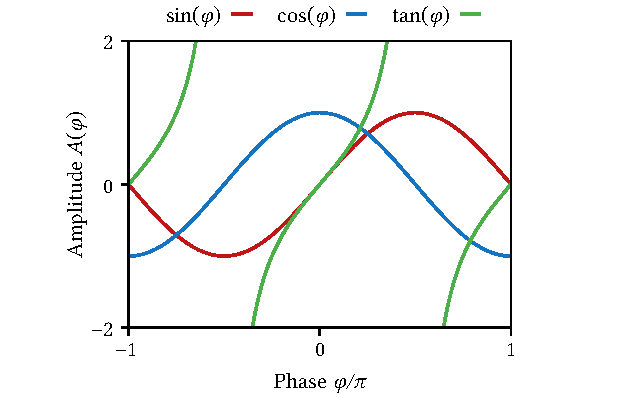
\includegraphics[width=\textwidth]{test.pdf}
  \caption
  {
    This is an example figure made by \textsc{gnuplot}. 
    I have also included an intentionally long caption to show the margins.
  }
  \label{fig:test}
\end{figure}

\section{Lorem ipsum}
\lipsum

    \chapter{Conclusion}\noindent
This would be a natural place to summarize your main results, and perhaps provide an outlook for future developments in the field.
 
  \backmatter
    \printbibliography
\end{document}
